\documentclass[a4paper,11pt]{article}
\pdfoutput=1 % if your are submitting a pdflatex (i.e. if you have
             % images in pdf, png or jpg format)
\usepackage{subcaption}

\usepackage{jinstpub} % for details on the use of the package, please
                     % see the JINST-author-manual
\usepackage{lineno}
\linenumbers
\def\myhyphen{{\hbox{-}}}
\usepackage{booktabs}
\usepackage{amsmath}
\title{\boldmath Cosmic-ray LArTPC reconstruction efficiency measurement using an external cosmic-muon counter}

\collaboration{The MicroBooNE Collaboration}

\author[g]{R.~Acciarri}
\author[z]{C.~Adams}
\author[h]{R.~An}
\author[w]{J.~Asaadi}
\author[a]{M.~Auger}
\author[g]{L.~Bagby}
\author[g]{B.~Baller}
\author[q]{G.~Barr}
\author[q]{M.~Bass}
\author[x]{F.~Bay}
\author[b]{M.~Bishai}
\author[j]{A.~Blake}
\author[i]{T.~Bolton}
\author[m]{L.~Bugel}
\author[f]{L.~Camilleri}
\author[f]{D.~Caratelli}
\author[g]{B.~Carls}
\author[g]{R.~Castillo~Fernandez}
\author[g]{F.~Cavanna}
\author[b]{H.~Chen}
\author[r]{E.~Church}
\author[l,f]{D.~Cianci}
\author[m]{G.~H.~Collin}
\author[m]{J.~M.~Conrad}
\author[u]{M.~Convery}
\author[f]{J.~I.~Crespo-Anad\'{o}n}
\author[q]{M.~Del~Tutto}
\author[j]{D.~Devitt}
\author[s]{S.~Dytman}
\author[u]{B.~Eberly}
\author[a]{A.~Ereditato}
\author[c]{L.~Escudero Sanchez}
\author[v]{J.~Esquivel}
\author[z]{B.~T.~Fleming}
\author[d]{W.~Foreman}
\author[l]{A.~P.~Furmanski}
\author[k]{G.~T.~Garvey}
\author[f]{V.~Genty}
\author[a]{D.~Goeldi}
\author[i]{S.~Gollapinni}
\author[s]{N.~Graf}
\author[z]{E.~Gramellini}
\author[g]{H.~Greenlee}
\author[e]{R.~Grosso}
\author[q]{R.~Guenette}
\author[z]{A.~Hackenburg}
\author[v]{P.~Hamilton}
\author[m]{O.~Hen}
\author[l]{J.~Hewes}
\author[l]{C.~Hill}
\author[d]{J.~Ho}
\author[i]{G.~Horton-Smith}
\author[g]{C.~James}
\author[c]{J.~Jan~de~Vries}
\author[y]{C.-M.~Jen}
\author[s]{L.~Jiang}
\author[e]{R.~A.~Johnson}
\author[m]{B.~J.~P.~Jones}
\author[b]{J.~Joshi}
\author[g]{H.~Jostlein}
\author[f]{D.~Kaleko}
\author[l,f]{G.~Karagiorgi}
\author[g]{W.~Ketchum}
\author[b]{B.~Kirby}
\author[g]{M.~Kirby}
\author[g]{T.~Kobilarcik}
\author[a]{I.~Kreslo}
\author[q]{A.~Laube}
\author[b]{Y.~Li}
\author[j]{A.~Lister}
\author[h]{B.~R.~Littlejohn}
\author[g]{S.~Lockwitz}
\author[a]{D.~Lorca}
\author[k]{W.~C.~Louis}
\author[a]{M.~Luethi}
\author[g]{B.~Lundberg}
\author[z]{X.~Luo}
\author[g]{A.~Marchionni}
\author[y]{C.~Mariani}
\author[c]{J.~Marshall}
\author[h]{D.~A.~Martinez~Caicedo}
\author[i]{V.~Meddage}
\author[o]{T.~Miceli}
\author[k]{G.~B.~Mills}
\author[m]{J.~Moon}
\author[b]{M.~Mooney}
\author[g]{C.~D.~Moore}
\author[n]{J.~Mousseau}
\author[l]{R.~Murrells}
\author[s]{D.~Naples}
\author[t]{P.~Nienaber}
\author[j]{J.~Nowak}
\author[g]{O.~Palamara}
\author[s]{V.~Paolone}
\author[o]{V.~Papavassiliou}
\author[o]{S.F.~Pate}
\author[g]{Z.~Pavlovic}
\author[l]{D.~Porzio}
\author[v]{G.~Pulliam}
\author[b]{X.~Qian}
\author[g]{J.~L.~Raaf}
\author[i]{A.~Rafique}
\author[u]{L.~Rochester}
\author[a]{C.~Rudolf~von~Rohr}
\author[z]{B.~Russell}
\author[d]{D.~W.~Schmitz}
\author[g]{A.~Schukraft}
\author[f]{W.~Seligman}
\author[f]{M.~H.~Shaevitz}
\author[a]{J.~Sinclair}
\author[g]{E.~L.~Snider}
\author[v]{M.~Soderberg}
\author[l]{S.~S{\"o}ldner-Rembold}
\author[q,1]{S.~R.~Soleti\note{Corresponding author.}}
\author[g]{P.~Spentzouris}
\author[n]{J.~Spitz}
\author[e]{J.~St.~John}
\author[g]{T.~Strauss}
\author[l]{A.~M.~Szelc}
\author[p]{N.~Tagg}
\author[f]{K.~Terao}
\author[c]{M.~Thomson}
\author[g]{M.~Toups}
\author[u]{Y.-T.~Tsai}
\author[z]{S.~Tufanli}
\author[u]{T.~Usher}
\author[k]{R.~G.~Van~de~Water}
\author[b]{B.~Viren}
\author[a]{M.~Weber}
\author[c]{J.~Weston}
\author[s]{D.~A.~Wickremasinghe}
\author[g]{S.~Wolbers}
\author[m]{T.~Wongjirad}
\author[o]{K.~Woodruff}
\author[g]{T.~Yang}
\author[g]{G.~P.~Zeller}
\author[d]{J.~Zennamo}
\author[b]{C.~Zhang}

% Institutions in alphabetical order
\affiliation[a]{Universit{\"a}t Bern, Bern CH-3012, Switzerland}
\affiliation[b]{Brookhaven National Laboratory (BNL), Upton, NY, 11973, USA}
\affiliation[c]{University of Cambridge, Cambridge CB3 0HE, United Kingdom}
\affiliation[d]{University of Chicago, Chicago, IL, 60637, USA}
\affiliation[e]{University of Cincinnati, Cincinnati, OH, 45221, USA}
\affiliation[f]{Columbia University, New York, NY, 10027, USA}
\affiliation[g]{Fermi National Accelerator Laboratory (FNAL), Batavia, IL 60510, USA}
\affiliation[h]{Illinois Institute of Technology (IIT), Chicago, IL 60616, USA}
\affiliation[i]{Kansas State University (KSU), Manhattan, KS, 66506, USA}
\affiliation[j]{Lancaster University, Lancaster LA1 4YW, United Kingdom}
\affiliation[k]{Los Alamos National Laboratory (LANL), Los Alamos, NM, 87545, USA}
\affiliation[l]{The University of Manchester, Manchester M13 9PL, United Kingdom}
\affiliation[m]{Massachusetts Institute of Technology (MIT), Cambridge, MA, 02139, USA}
\affiliation[n]{University of Michigan, Ann Arbor, MI, 48109, USA}
\affiliation[o]{New Mexico State University (NMSU), Las Cruces, NM, 88003, USA}
\affiliation[p]{Otterbein University, Westerville, OH, 43081, USA}
\affiliation[q]{University of Oxford, Oxford OX1 3RH, United Kingdom}
\affiliation[r]{Pacific Northwest National Laboratory (PNNL), Richland, WA, 99352, USA}
\affiliation[s]{University of Pittsburgh, Pittsburgh, PA, 15260, USA}
\affiliation[t]{Saint Mary's University of Minnesota, Winona, MN, 55987, USA}
\affiliation[u]{SLAC National Accelerator Laboratory, Menlo Park, CA, 94025, USA}
\affiliation[v]{Syracuse University, Syracuse, NY, 13244, USA}
\affiliation[w]{University of Texas, Arlington, TX, 76019, USA}
\affiliation[x]{TUBITAK Space Technologies Research Institute, METU Campus, TR-06800, Ankara, Turkey}
\affiliation[y]{Center for Neutrino Physics, Virginia Tech, Blacksburg, VA, 24061, USA}
\affiliation[z]{Yale University, New Haven, CT, 06520, USA}


\emailAdd{stefano.soleti@physics.ox.ac.uk}




\abstract{The MicroBooNE experiment is a liquid argon TPC experiment designed for short-baseline neutrino physics, currently running at Fermilab. Due to its location near the surface, cosmic muons can be a source of backgrounds to several analyses and a good understanding of them is of fundamental importance for the experiment. This study presents a method of using an external muon counter system to determine the cosmic-ray reconstruction efficiency in MicroBooNE.
Data has been acquired with the external muon counter system placed in the three different positions, corresponding to cosmic rays hitting different parts of the LArTPC.
The reconstruction of the tracks is performed using the multi-algorithm Pandora framework. The data reconstruction efficiency is $\epsilon_{\mathrm{data}}=96.1\pm0.1~(\mathrm{stat}) \pm 1.1~(\mathrm{sys})\%$, in good agreement with the Monte Carlo reconstruction efficiency $\epsilon_{\mathrm{MC}} = 96.3\pm0.1\%$.
This analysis represents a small-scale demonstration of the method that can be used with the data coming from the recently installed Cosmic Ray Tagger, which is able to tag $\sim80\%$ of the cosmic rays passing through the MicroBooNE detector.}

\keywords{Time projection chambers; Pattern recognition, cluster finding, calibration and fitting methods; Performance of High Energy Physics Detectors}


\arxivnumber{1234.56789} % only if you have one



\begin{document}
\maketitle
\flushbottom

\section{Introduction}
\label{sec:intro}
MicroBooNE (Micro Booster Neutrino Experiment) is an R&D experiment based at the Fermi National Accelerator Laboratory (Fermilab) that uses a large Liquid Argon Time Projection Chamber (LArTPC) to investigate the excess of low energy events observed by the MiniBooNE experiment [1] and to study neutrino-argon cross-sections. MicroBooNE is part of the Short-Baseline Neutrino (SBN) physics program, along with two other LArTPCs: the Short Baseline Near Detector (SBND)and the Imaging Cosmic And Rare Underground Signal (ICARUS) detector. MicroBooNE also provides important research and development in terms of detector technology and event reconstruction techniques for future LArTPC experiments including DUNE (Deep Underground Neutrino Experiment).

The MicroBooNE detector[2] consists of a rectangular time projection chamber (TPC) with dimensions 2.6 m width × 2.3 m height × 10.4 m length located 470 m away from the Booster Neutrino Beam (BNB) target. LArTPCs allow for precise three-dimensional reconstruction of particle interactions. The x− direction of the TPC corresponds to the drift coordinate, the y− direction is the vertical direction, and the z− direction is the direction along the beam. The mass of active liquid argon in the MicroBooNE TPC is 89 tons, with the total cryostat containing 170 tons of liquid argon.

A set of 32 photomultiplier tubes (PMTs) and three wire planes with 3 mm spacing at angles of 0, and ± 60 degrees with respect to the vertical are located in the TPC for event reconstruction (Fig-ure 1), and the cathode plane operating voltage is -70 kV. In a neutrino interaction, a neutrino from the beam interacts with an argon nucleus and the charged outgoing secondary particles traverse the medium, losing energy and leaving an ionization trail. The resulting ionization electrons drift to the anode side of the TPC, containing the wire planes. The passage of these electrons near the first two wire planes induces a signal in them and their collection on the third plane also generates a signal. These signals are used to create three distinct two-dimensional views (in terms of wire and time) of the event. Combining these wire signals with timing information from the PMTs allows for full three-dimensional reconstruction of the event. The fiducial volume used in this analysis is defined as the full TPC volume reduced by 20 cm from both the cathode plane and the anode wire planes, by 26.5 cm from both the top and bottom walls of the TPC, by 20 cm from the beam-upstream wall of the TPC, and by 36.8 cm from the beam-downstream wall of the TPC, which corresponds to a mass of 55 tons.

The Booster Neutrino Beam (BNB) is predominantly composed of muon neutrinos (νμ) with a peak neutrino energy of about 0.7 GeV, which can undergo charge-current (νμCC) interactions in the TPC and produce muons. For muon tracks that are completely contained in the TPC, it is straightforward to calculate their momentum with a measurement of the length of the particle’s track, or with calorimetric measurements which come from wire signal measurements. However, around half of muons from BNB neutrino events in MicroBooNE are not fully contained in the TPC, and therefore using length-based calculations for these uncontained tracks is not a possibility. The only way to compute the energy of a non-contained three-dimensional track is by means of multiple coulomb scattering (MCS).

This paper describes the work done to study the reconstruction efficiencies using a dataset of cosmic rays in the MicroBooNE TPC passing through the Muon Counter System (MuCS). The goal is to provide data and Monte Carlo reconstruction efficiencies that can be used to compare reconstruction performances and to show that an external cosmic-ray counter can be used to measure the data reconstruction efficiency in MicroBooNE.

We measured the data reconstruction efficiency comparing the number of events triggered by the MuCS and the number of events with a MuCS-compatible reconstructed track.
The Monte Carlo reconstruction efficiency, instead, was measured by comparing the number of generated cosmic rays with the number of reconstructed tracks, using simulated cosmic rays hitting the entire TPC.

The reconstruction efficiency is expressed as a function of the cosmic-ray starting angle (given by the spherical angles $\theta$ and $\phi$ relative to the orientation of the cosmic-ray trajectory) and of the expected length $L$ of its path in the TPC. More details on the Monte Carlo generation can be found in Sec. \ref{sec:merging}.%, assuming it is a minimum-ionizing particle (MIP).

Using the \texttt{pan\-do\-ra\-Co\-smic} algorithm \cite{pandoracosmic} provided by the Pandora framework \cite{pandora}, the overall reconstruction efficiency is $96.1\pm0.1\thinspace(\mathrm{stat}) \pm 1.1\thinspace(\mathrm{sys})\thinspace\%$ for data and $96.3\pm0.1\thinspace\%$ for Monte Carlo.

In the future, the method described in this paper will be adapted to use the data coming form the Cosmic Ray Tagger \cite{crt}, which is able to tag around 80\% of the cosmic rays hitting MicroBooNE LArTPC. In this way, we will be able to cover the entire $(\theta,\phi,L)$ parameter space and measure efficiency-corrected quantities, such as the cosmic-ray flux in the LArTPC.


\section{The Muon Counter System}\label{sec:proc}
The MuCS consists of two sets of planar modules made up of scintillator strips placed into two separate, light-tight panels, readout via wavelength shifting fibers connected to Multi-Anode PMTs and placed on the top of the TPC. The Multi-Anode PMTs are readout by a DAQ system, separated from the DAQ system that reads out the TPC and PMT systems of the main detector.

Each planar module is made up of two sets of 24 scintillator strips, 4 cm wide, arranged into bi-layers oriented perpendicular to each other. This configuration provides two coordinates ($z$ and $x$ in the MicroBooNE TPC coordinate system, shown in Fig. \ref{fig:coord}) of the crossing points of the cosmic rays. Combining these two coordinates with the height of the modules (corresponding to the $y$ coordinate in the MicroBooNE TPC coordinate system), it is possible to extrapolate the three-dimensional trajectory of the cosmic ray.

The starting angle of the cosmic ray, in spherical coordinates, will be given by:
\begin{align}
  \theta = \mathrm{acos}\left(\frac{z_{\mathrm{top}}-z_{\mathrm{bottom}}}{r}\right) \\
  \phi = \mathrm{atan}\left(\frac{y_{\mathrm{top}}-y_{\mathrm{bottom}}}{x_{\mathrm{top}}-x_{\mathrm{bottom}}}\right),
\end{align}
where $r = \sqrt{(x_{\mathrm{top}}-x_{\mathrm{bottom}})^2+(y_{\mathrm{top}}-y_{\mathrm{bottom}})^2+(z_{\mathrm{top}}-z_{\mathrm{bottom}})^2}$ and the top (bottom) coordinates are given by the hits in the top (bottom) MuCS panel.
\begin{figure}[htbp]
  \begin{center}
    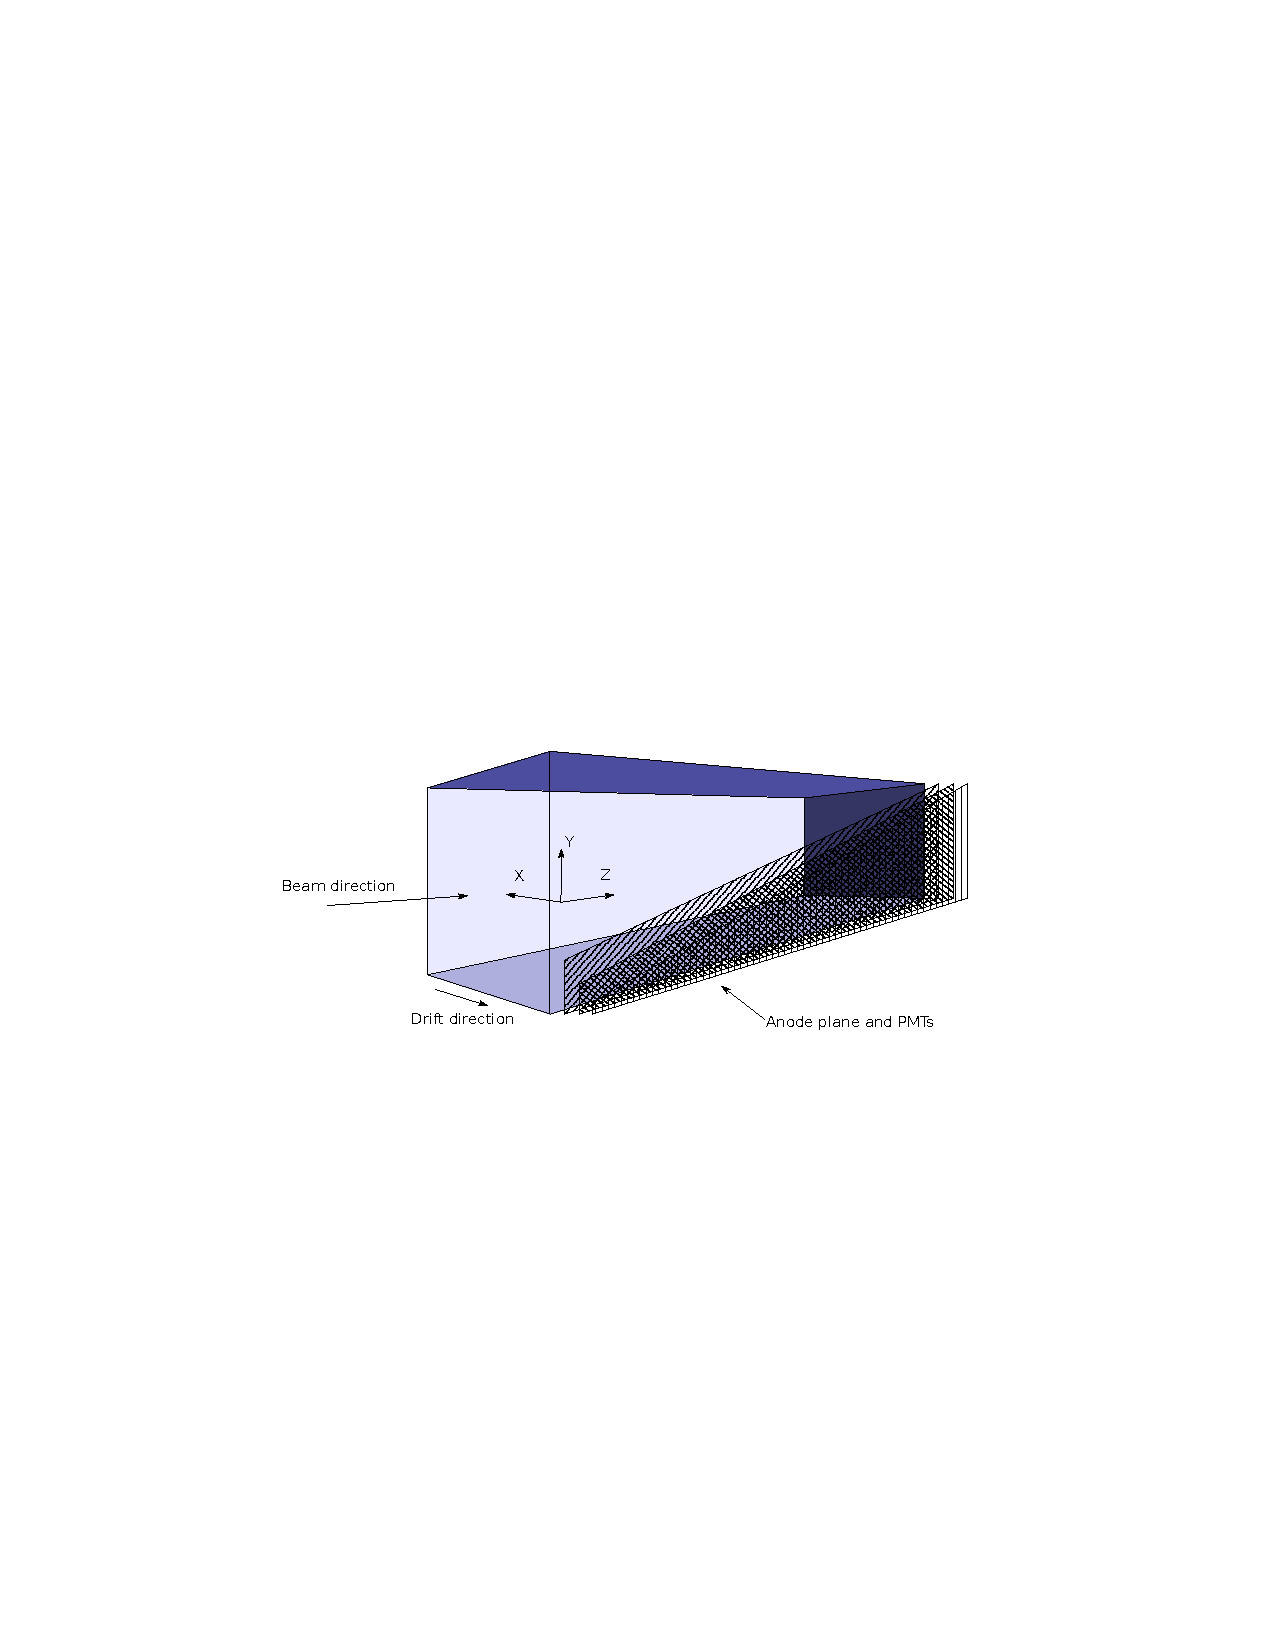
\includegraphics[width=0.8\linewidth]{figures/coord.pdf}

    \caption{The MicroBooNE coordinate system. The three wire planes are vertical (collection plane) and at  $\pm60^{\circ}$ to the vertical (induction planes). The dimensions of the TPC are 256.35 cm $\times$ 233 cm $\times$ 1036.8 cm (x $\times$ y $\times$ z). The fiducial volume of the detector is 236.35 cm $\times$ 203 cm $\times$ 1026.8 cm. The coordinate system is explained in detail in \cite{mcdata}.} \label{fig:coord}
  \end{center}
\end{figure}

This analysis has been performed on three merged datasets, acquired with different geometrical configurations. For the three different configurations, the two panels have been placed at the upstream end, at the center and at the downstream end of MicroBooNE, respectively.

A three-dimensional schematic of the three MuCS setups is shown in Fig. \ref{fig:mucs} and the coordinates of the two panels for each configuration are reported in Tab. \ref{tab:mucs}.
\begin{figure}[htbp]
  \begin{subfigure}{0.30\textwidth}
    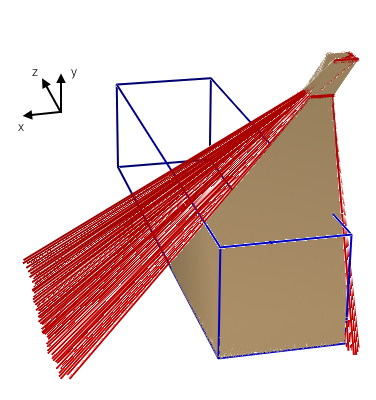
\includegraphics[width=\linewidth]{figures/upstream.png}
    \caption{Upstream} \label{fig:upstream}
  \end{subfigure}
  \begin{subfigure}{0.30\textwidth}
    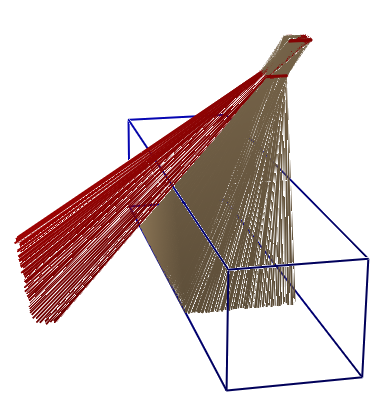
\includegraphics[width=\linewidth]{figures/center.png}
    \caption{Center} \label{fig:centre}
  \end{subfigure}
  \begin{subfigure}{0.30\textwidth}
    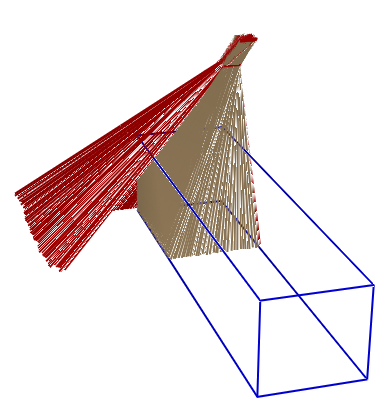
\includegraphics[width=\linewidth]{figures/downstream.png}
    \caption{Downstream} \label{fig:downstream}
  \end{subfigure}

  \caption{Monte Carlo simulation of the possible MuCS trajectories in the three different MuCS setups used in this analysis. Brown tracks correspond to cosmic rays hitting both MuCS panels and the TPC, while red tracks go through only the MuCS and miss the TPC.} \label{fig:mucs}
\end{figure}

\begin{table}[htbp]
  \centering
  \begin{tabular}{lcrrrccccc}
    \toprule
    \textbf{Configuration} & \phantom{abc}& \multicolumn{2}{c}{x [cm]} & \phantom{abc} & \multicolumn{2}{c}{y [cm]} & \phantom{abc} & \multicolumn{2}{c}{z [cm]}\\
    \cmidrule{3-4} \cmidrule{6-7} \cmidrule{9-10}
    & & start & end & & start & end & & start & end\\
    \midrule

    \textbf{Upstream} & & & & & & & & & \\
    Top panel & & -75 & -27 & & 392 & 393 & & 224 & 272\\
    Bottom panel & & -27 & 21 & & 320 & 321 & & 224 & 272\\

    \midrule
    \textbf{Center} & & & & & & & & & \\
    Top panel & & -72 & -24 & & 397 & 398 & & 579 & 627\\
    Bottom panel & & -27 & 21 & & 320 & 321 & & 581 & 629\\
    \midrule
    \textbf{Downstream} & & & & & & & & & \\
    Top panel & & -75 & -27 & & 392 & 393 & & 971 & 1019\\
    Bottom panel & & -27 & 21 & & 320 & 321 & & 971 & 1019\\
    \bottomrule

  \end{tabular}
  \caption{Coordinates of the top and bottom panels of the MuCS detector for three geometrical configurations, expressed in the TPC coordinate reference frame.}\label{tab:mucs}
\end{table}

\section{MuCS Merging}\label{sec:merging}
The MuCS is designed to provide a trigger on through-going muons that intersect two planes of scintillator strips. The trigger is propagated to the MicroBooNE trigger board to record a full TPC and PMT readout. With the MuCS trigger in place, the $t_0$ for a track associated with the MuCS is known and these tracks are useful for various detector physics and reconstruction studies.

The dataset used for this study has been collected with the DAQ configured in the trigger-readout mode: the MuCS trigger is sent to the TPC readout, while the MuCS DAQ saves the hit patterns seen in the scintillator strips.
The MuCS triggers at a rate of nearly 3 Hz.
Given a DAQ integration window of 100 ns, the accidental coincidental rate is negligible for our study. The probability that, during the same readout window (4.8 ms), another cosmic ray hits the MuCS is, given a trigger rate of 3 Hz, 0.01\% and it has also been considered negligible.

The data then follows a processing path that merges the MuCS hit patterns and extrapolated trajectory information with the TPC and PMT data stream to form a MuCS-merged dataset. A flowchart of the procedure is shown in Fig. \ref{fig:scheme}.

\begin{figure}[htbp]
  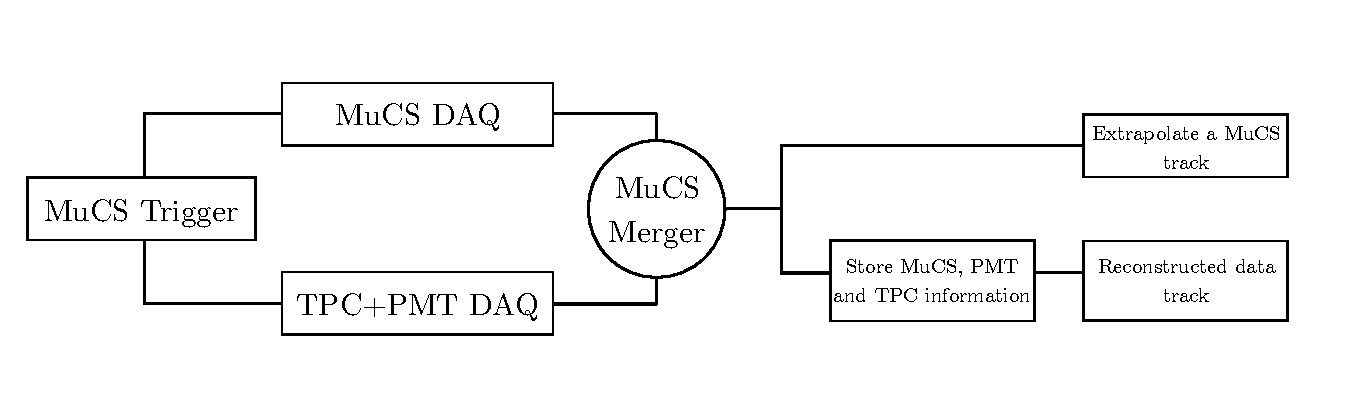
\includegraphics[width=\linewidth]{figures/scheme.pdf}
  \caption{Flowchart showing the procedure used to generate the dataset used in this analysis. We end up with two data products: one with extrapolated coordinates obtained using MuCS-only data and one with reconstructed TPC tracks and PMT flashes, if present.} \label{fig:scheme}
\end{figure}

The hits in the MuCS are used to obtain a point for each panel and extrapolate a track (MuCS-extrapolated track). The TPC hits, instead, are fed to the MicroBooNE reconstruction chain: the reconstructed track with the closest starting point to the intersection of the MuCS-extrapolated track with the TPC is stored in the dataset and it is defined as a MuCS-tagged track. The distance $d$ between these two points is defined as:
\begin{equation}\label{eq:d}
d = \sqrt{(x_{\mathrm{MuCS}}-x_{\mathrm{reco}})^2+(y_{\mathrm{MuCS}}-y_{\mathrm{reco}})^2+(z_{\mathrm{MuCS}}-z_{\mathrm{reco}})^2},
\end{equation}
where $(x_{\mathrm{MuCS}},y_{\mathrm{MuCS}},z_{\mathrm{MuCS}})$ and $(x_{\mathrm{reco}},y_{\mathrm{reco}},z_{\mathrm{reco}})$ are the coordinates of the intersection of the MuCS-extrapolated track with the TPC and of the start of the closest reconstructed track, respectively.
A PMT flash is associated with the MuCS signal if it falls between -1.0 and -0.8 \textmu s, where $t=0$ is given by the MuCS signal.
Fig. \ref{fig:evd} shows a diagram with the MuCS-tagged track, the MuCS-extrapolated track and the other reconstructed tracks in the same readout window.

\begin{figure}[htbp]
  \begin{center}
  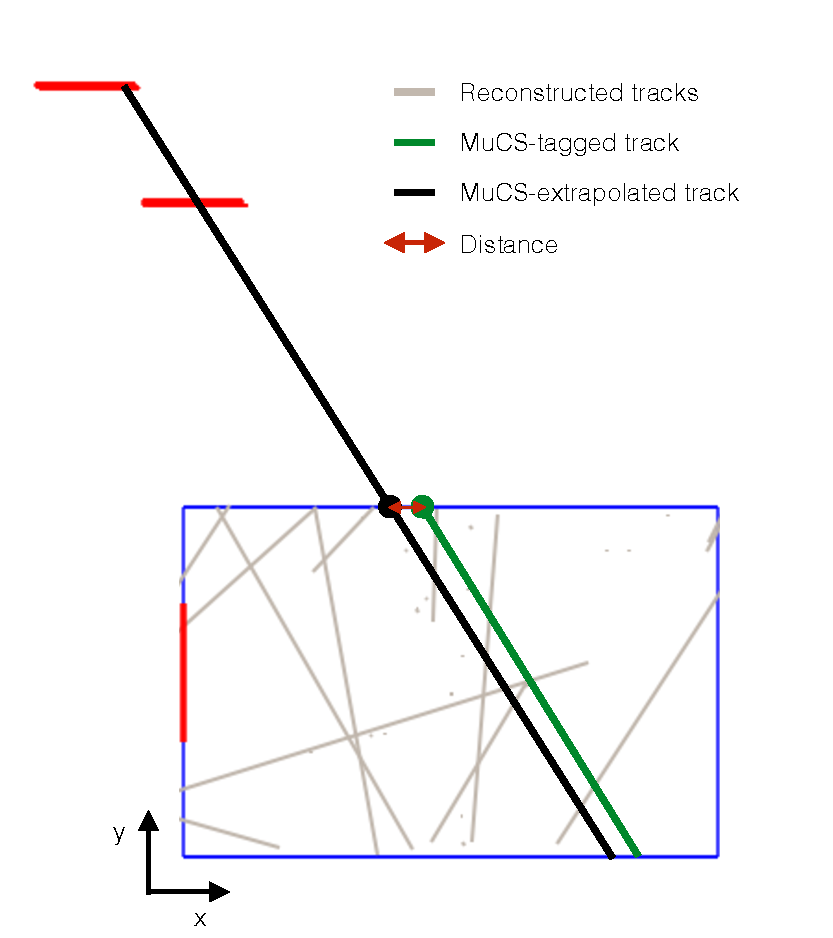
\includegraphics[width=0.50\linewidth]{figures/evd.pdf}  \vspace{1.8em}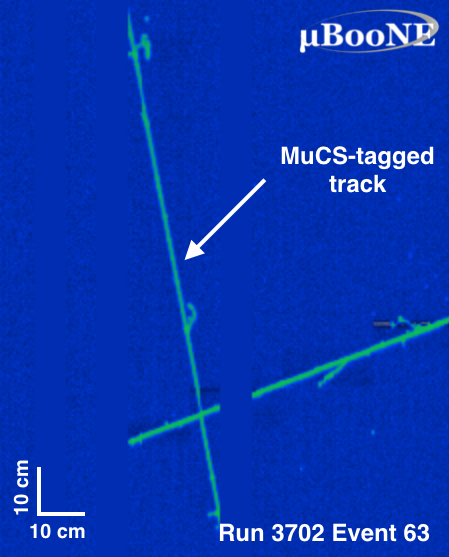
\includegraphics[width=0.40\linewidth]{figures/evd_display.png}

  \caption{Left: bi-dimensional view of a MuCS event. The black line shows the MuCS-extrapolated track, while the green line correspond to the MuCS-tagged track. The black and green points correspond to the $(x_{\mathrm{MuCS}},y_{\mathrm{MuCS}},z_{\mathrm{MuCS}})$ and $(x_{\mathrm{reco}},y_{\mathrm{reco}},z_{\mathrm{reco}})$ coordinates, respectively. The red vertical line on the left border correspond to the position of the PMT flash associated to the MuCS-tagged track. Right: corresponding portion of the event display for the collection plane, showing the MuCS-tagged track.} \label{fig:evd}
\end{center}
\end{figure}

Our dataset will then include two different sets of information, with a one-to-one correspondence:
\begin{itemize}
  \item MuCS-extrapolated information: using the two points given by the MuCS (one for each panel) we extrapolate a line crossing the entire TPC. In this way we obtain two extrapolated starting angles ($\theta$ and $\phi$), an extrapolated track length $L$ and extrapolated start/end points, using only MuCS information.
  \item Reconstructed TPC data information: for each event, we store the reconstructed spatial information of the MuCS-tagged track and of the in-time PMT flash, if present.
\end{itemize}


As Monte Carlo sample we used a complete MCC7 cosmic-ray simulation, as described in \cite{cosmic}. The cosmic rays have been generated using CORSIKA \cite{corsika},  propagated with GEANT4 \cite{geant}, and then passed through the detector simulation stage. The detector simulation attempts to simulate the detector response as precisely as possible, meaning that the current state of the detector is reflected, including known unresponsive and noisy wires. Other known effects, such as the space charge effect \cite{sce}, are not currently modeled in the simulation.

The spherical angles $\theta$ and $\phi$ are measured using the starting point in the TPC and direction of the generated cosmic ray, while the expected track length $L$ is measured extrapolating a line through the TPC.
The distance $d$ is defined in this case as:
\begin{equation}\label{eq:d_mc}
d = \sqrt{(x_{\mathrm{sim}}-x_{\mathrm{reco}})^2+(y_{\mathrm{sim}}-y_{\mathrm{reco}})^2+(z_{\mathrm{sim}}-z_{\mathrm{reco}})^2},
\end{equation}
where $(x_{\mathrm{sim}},y_{\mathrm{sim}},z_{\mathrm{sim}})$ and $(x_{\mathrm{reco}},y_{\mathrm{reco}},z_{\mathrm{reco}})$ are the coordinates of the intersection of the simulated cosmic-ray trajectory with the TPC and of the closest reconstructed track, respectively.

From this complete Monte Carlo simulation, then, we selected only the cosmic rays with a starting angle $(\theta,\phi)$ within the geometrical acceptance of the MuCS.

Our aim is to show that the reconstruction efficiency of simulated cosmic rays, generated all over the TPC, can be successfully compared to the data reconstruction efficiency, obtained placing a small muon counter system in three different places.

\acknowledgments

This is the most common positions for acknowledgments. A macro is
available to maintain the same layout and spelling of the heading.



% We suggest to always provide author, title and journal data:
% in short all the informations that clearly identify a document.

\begin{thebibliography}{99}

  \bibitem{pandoracosmic} R. Acciarri, et al. [MicroBooNE Collaboration], \textit{The Pandora multi-algorithm approach to automated pattern recognition in LAr TPC detectors}. \texttt{MICROBOONE- NOTE-1015-PUB}, 2016. \url{http://www-microboone.fnal.gov/publications/publicnotes/index.html}.

  \bibitem{pandora} J.~S.~Marshall and M.~A.~Thomson, \textit{The Pandora Software Development Kit for Pattern Recognition}, Eur.\ Phys.\ J.\ C 75, no. 9, 439 (2015) \texttt{doi:10.1140/epjc/s10052\-015-3659-3} \texttt{[arXiv:1506.05348 [physics.data-an]]}.

  \bibitem{crt} M. Auger, et al., \textit{A Novel Cosmic Ray Tagger System for Liquid Argon TPC Neutrino Detectors}, submitted to Instruments, \texttt{arXiv:1612.04614 [physics.ins-det]}.

  \bibitem{mcdata} R. Acciarri, et al. [MicroBooNE Collaboration], \textit{A Comparison of Monte-Carlo Simulations and Data from MicroBooNE}, \texttt{MICROBOONE-NOTE-1014-PUB}, 2016. \url{http:// www-microboone.fnal.gov/publications/publicnotes/index.html}.

  \bibitem{cosmic} R. Acciarri, et al. [MicroBooNE Collaboration], \textit{Cosmic Shielding Studies at MicroBooNE}. \texttt{MICROBOONE-NOTE-1005-PUB}, 2016. \url{http:// www-microboone.fnal.gov/publications/publicnotes/index.html}.

  \bibitem{corsika} D.~Heck, et al.,
  \textit{CORSIKA: A Monte Carlo code to simulate extensive air showers},
  \texttt{FZKA-6019}, 1998.

  \bibitem{geant} S.~Agostinelli, et al. [GEANT4 Collaboration], \textit{GEANT4: A Simulation toolkit}, Nucl.\ Instrum.\ Meth.\ A {506}, 250 (2003).

  \bibitem{sce} R. Acciarri, et al. [MicroBooNE Collaboration], \textit{Space Charge Effect Measurements and Corrections}. \texttt{MICROBOONE-NOTE-1018-PUB}, 2016. \url{http: //www-microboone.fnal.gov/publications/publicnotes/index.html}.

  \bibitem{besiii} W.~L.~Yuan, et al., \textit{Study of tracking efficiency and its systematic uncertainty from $J/\psi \to p \overline{p} \pi^+ \pi^-$ at BESIII}, Chin.\ Phys.\ C 40 (2016) no.2,  026201 \texttt{doi:10.1088/1674-1137/40/2/026201 [arXiv:1507.03453 [hep-ex]]}.

  \bibitem{pdg} C.~Patrignani, et al. [Particle Data Group Collaboration], \textit{Review of Particle Physics}, Chin.\ Phys.\ C 40 (2016) no.10,  100001 \texttt{doi:10.1088/1674-1137/40/10/100001}.


% Please avoid comments such as "For a review'', "For some examples",
% "and references therein" or move them in the text. In general,
% please leave only references in the bibliography and move all
% accessory text in footnotes.

% Also, please have only one work for each \bibitem.


\end{thebibliography}
\end{document}
